\documentclass[9pt]{IEEEtran}

\usepackage[english]{babel}
\usepackage{graphicx}
\usepackage{caption}
\captionsetup{justification=justified}

\usepackage{placeins}
\usepackage{epstopdf}
\usepackage{fancyhdr}
\usepackage{amsmath}
\usepackage{amsthm}
\usepackage{amssymb}
\usepackage{url}
\usepackage{array}
\usepackage{textcomp}
\usepackage{listings}
\usepackage{hyperref}
\usepackage{xcolor}
\usepackage{colortbl}
\usepackage{float}
\usepackage{gensymb}
\usepackage{longtable}
\usepackage{supertabular}
\usepackage{multicol}
\usepackage[justification=centering]{caption}
\usepackage{amsmath}
\usepackage{subcaption}

\usepackage[T1]{fontenc}
\usepackage{lmodern}
\input{glyphtounicode}
\pdfgentounicode=1

\graphicspath{{./figures/}}
\DeclareGraphicsExtensions{.pdf,.png,.jpg,.eps}

% correct bad hyphenation here
\hyphenation{op-tical net-works semi-conduc-tor trig-gs}

% ============================================================================================

\title{\vspace{0ex} Kalman Update and Particle Filter}

\author{Aljaž Konec\vspace{-4.0ex}}

% ============================================================================================

\begin{document}

\maketitle

\section{Introduction}

Kalman filter is a recursive Bayes filter that estimates the state of a linear dynamic system from a series of noisy measurements.
In this report we showcase its use for visual object tracking using a Particle filter.

In the first section we showcase Kalman filtering on three motion models: random walk, nearly constant velocity and nearly constant acceleration model.
Next, we implement a Particle filter that uses a Nearly constant velocity model and represents the target with a Color histogram.
Our implementation achieves an average overlap of 0.52 and 37 failures with 83 FPS on the VOT2014 dataset.

\section{Kalman Filter}
As mentioned before, we implemented the Kalman filter on three different motion models. 
Each model has two parameters, the system covariance noise $q$ and the observation covariance noise $r$.
These parameters quantify the uncertainty in the motion model prediction and the observation model respectively.
A higher value of $q$ means that the covariance matrix has larger values, which means that the motion model is more uncertain.
The same goes for the observation covariance noise $r$.
All matrixes are show in the appendix.
Since we have discrete time steps, we set the time step $T=1$ for the following examples of the motion models.

Figure \ref{fig:kalman} shows the performance of all three models with different values of $q$ and $r$.
It can be obseved that for all models, having high covariance of the observations (i.e. high $r$) results in the biggest divergances from the true state (true states are depicted in red in the Figure).
The Random walk model is the most sentitive to this parameter as it does not carry information about the velocity or acceleration both of which can help in better estimation of the true state.
Since the true state goes in a spiral, some variance in the system noise $q$ is needed as to allow for the change in direction.
This can be seen when we set $q=1$, the filter does not follow the true state as well as when $q=5$ with $r=1$ for both scenarios.

\subsection*{Kalman filter on jagged trajectory}
\begin{figure}[h!]
    \centering
    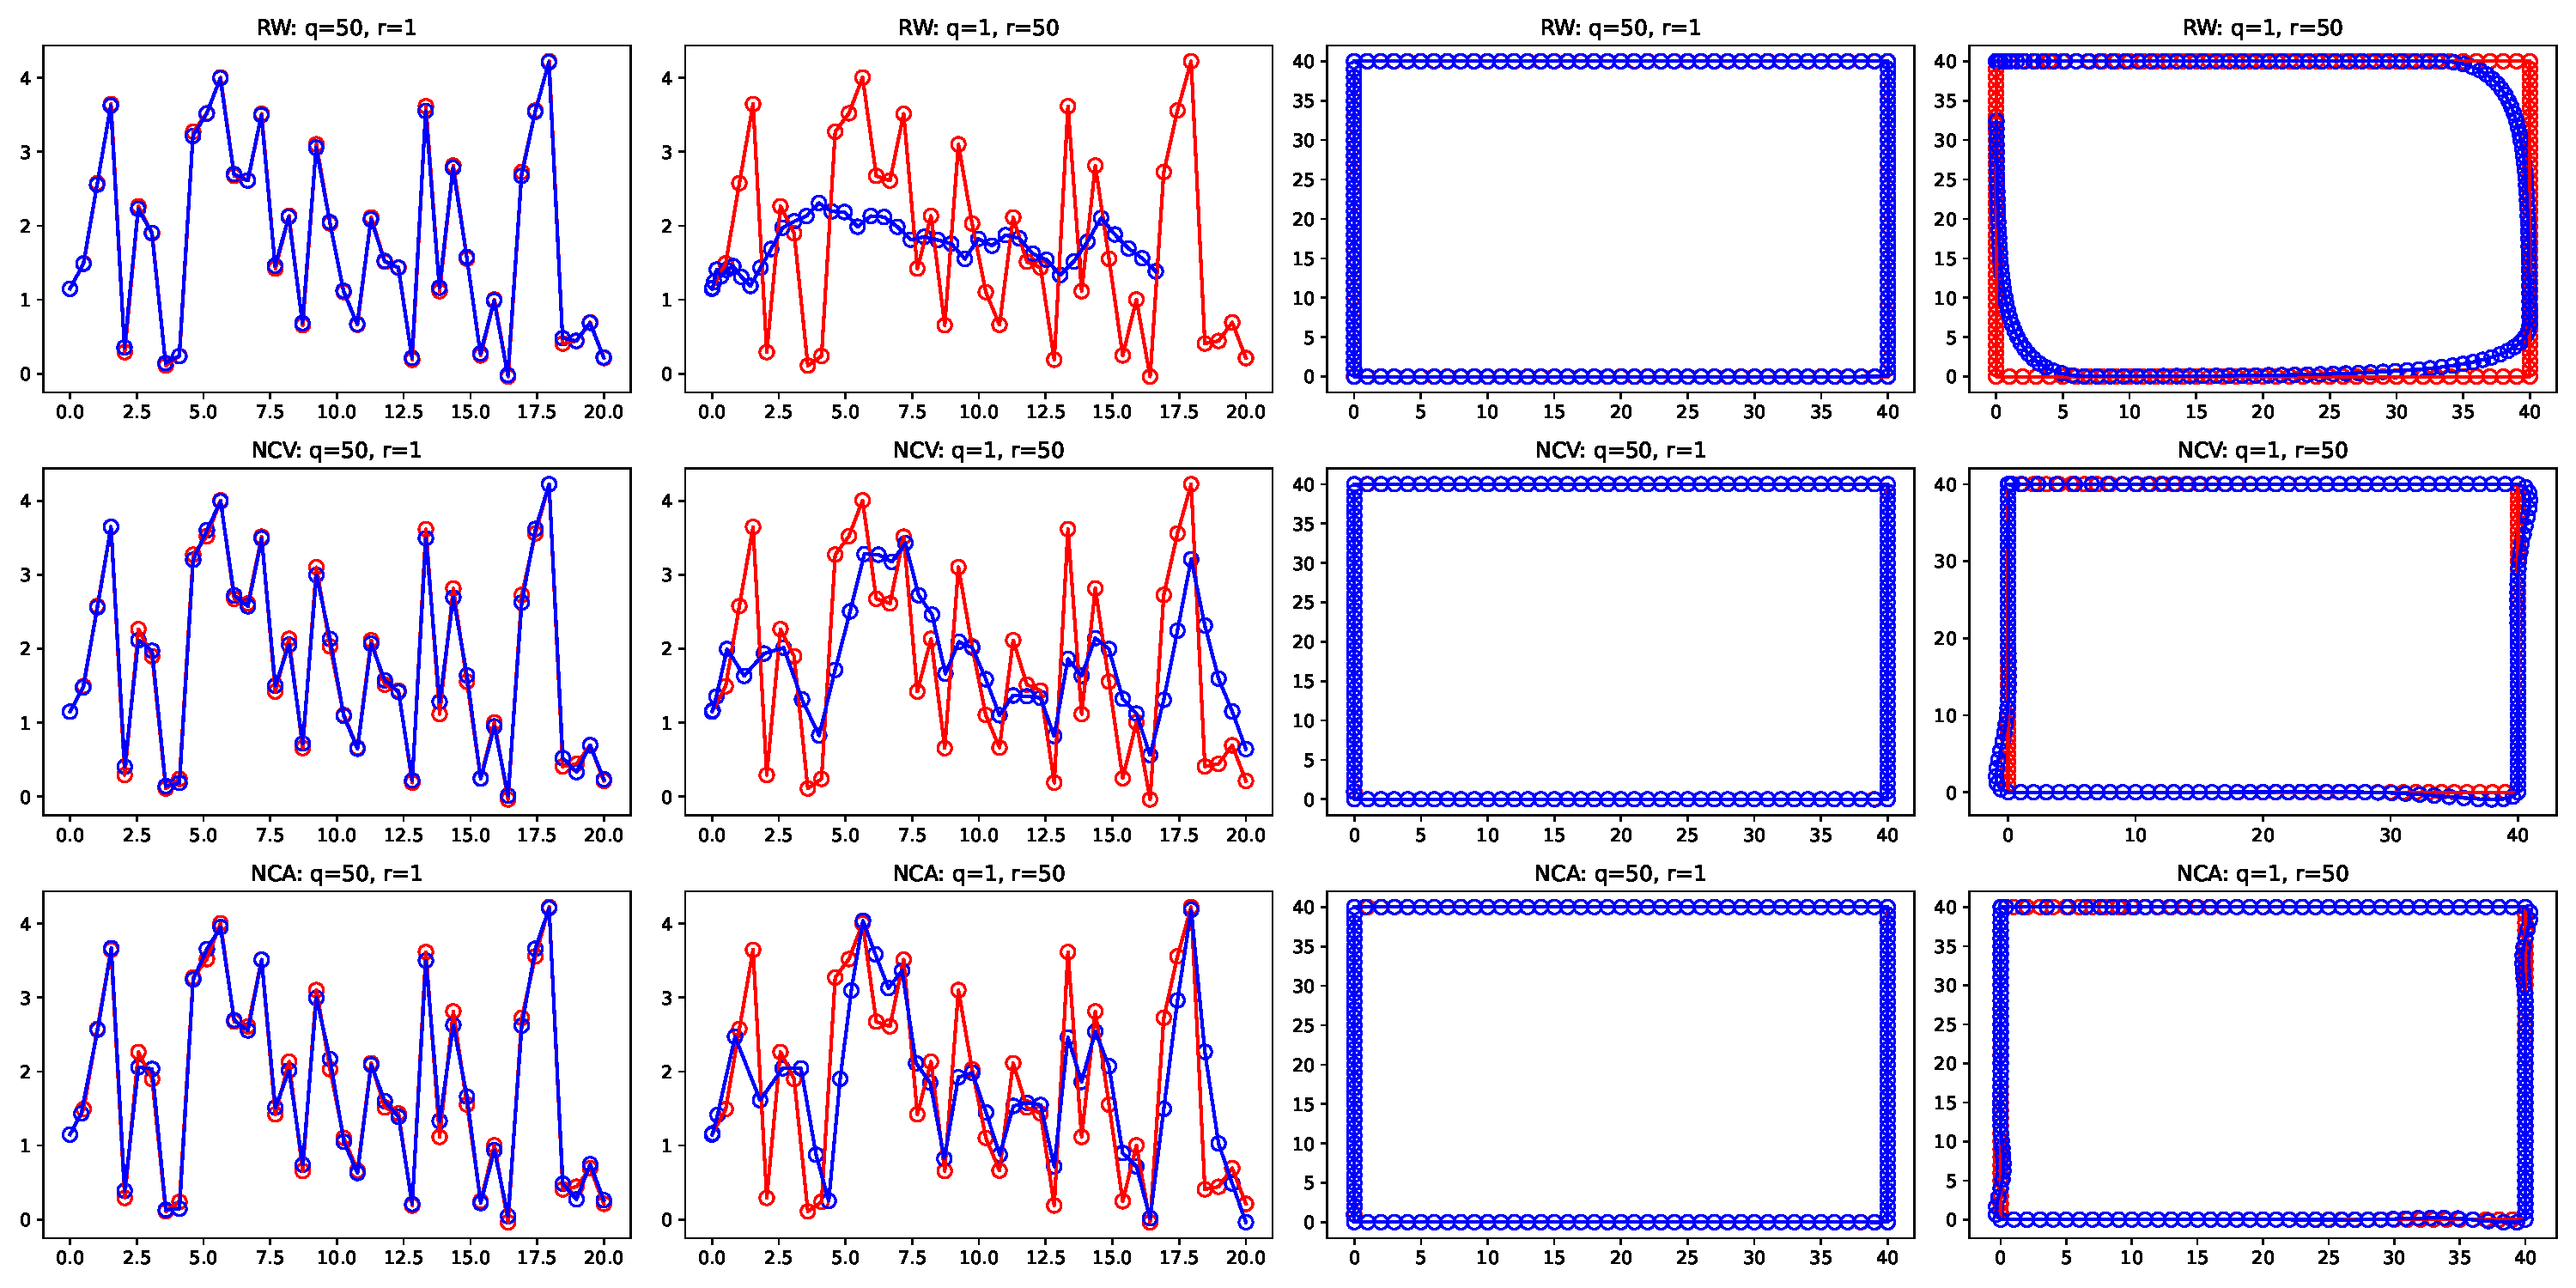
\includegraphics[width=0.48\textwidth]{kalman_filter_other.pdf}
    \caption{Kalman filter performance on jagged curves.}
    \label{fig:jagged}
\end{figure}

Figure \ref{fig:jagged} shows how the Kalman filter performs when the true state has more jagged trajectories.
We showcase two curves, one being a square and the other a jagged curve $y = x \mod 4 + w_{noise}$, where $w_{noise} \sim \mathcal{N}(0, 1) $ 
Similarly to the previous example, having very high confidence in our observations (i.e. low $r$) and low confidence in our motion model (i.e. high $q$) results better tracking of the true state.
The benefits of having a more complex motion model can be seen in the jagged curve when $q=1$ and $r=50$.
Each next model with a higher complexity performs better than the previous one.
The nearly constant acceleration model performs the best, as it can capture the sudden changes in the trajectory better than the other two models.
While the random walk model does not follow the true state at all.

\begin{figure*}
    \centering
    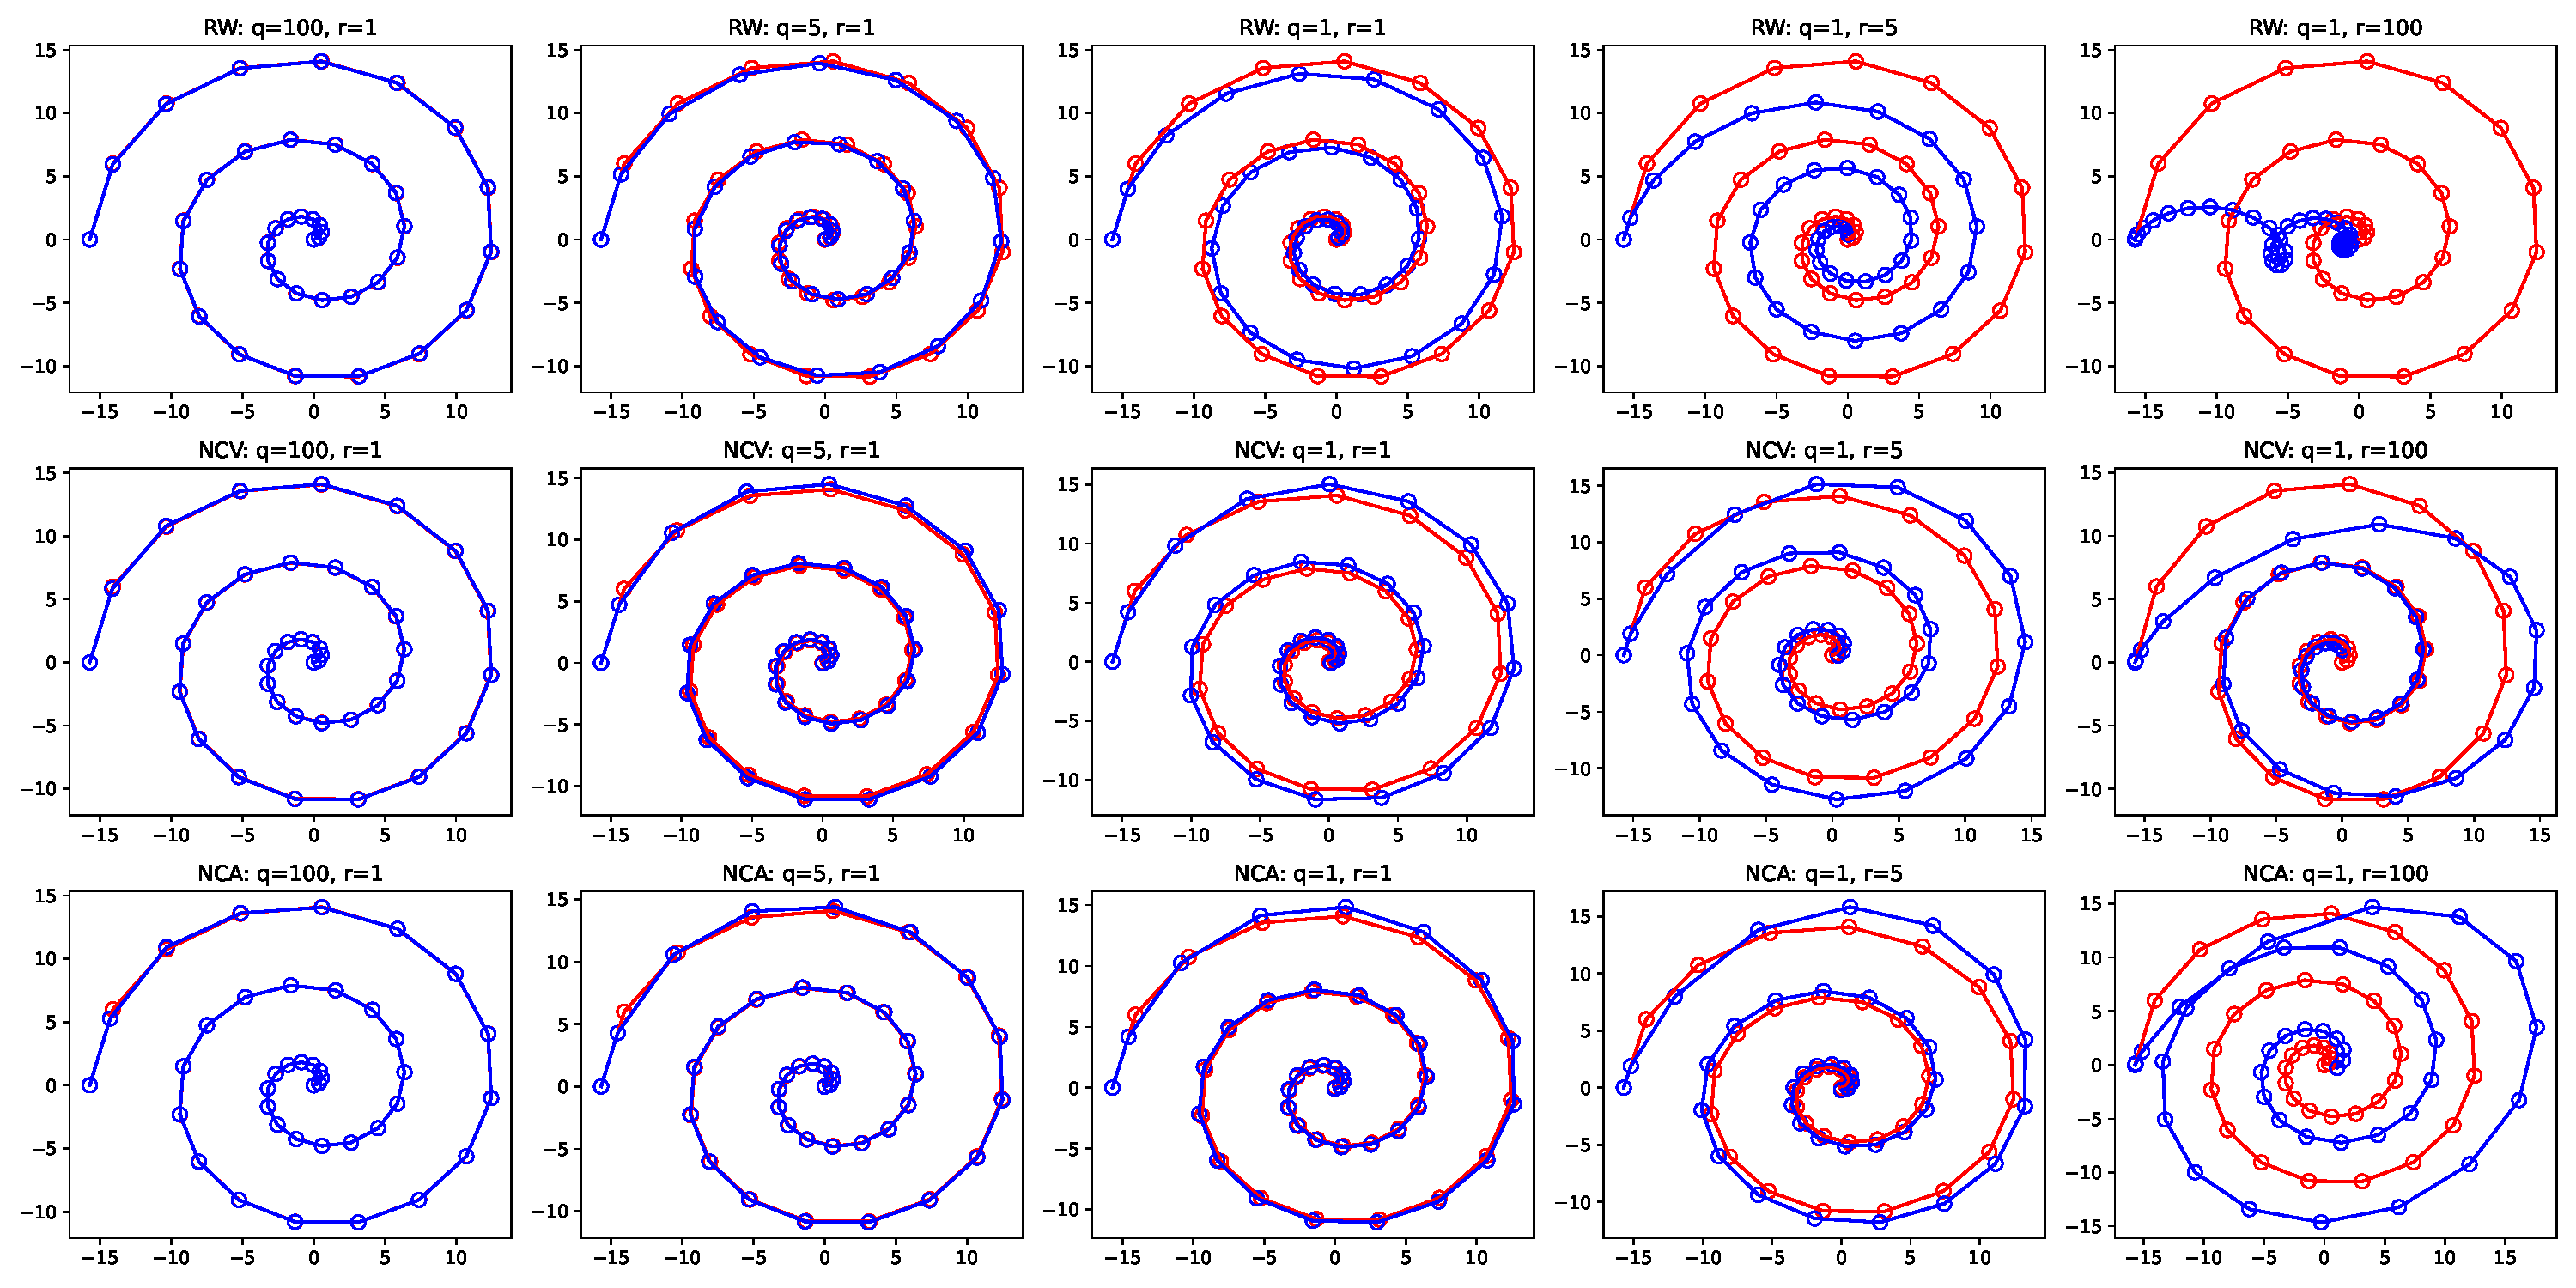
\includegraphics[width=\textwidth]{kalman_filter.pdf}
    \caption{Kalman filter performance using three different motion models.}
    \label{fig:kalman}
\end{figure*}



\section{Particle Filter}
In this section we discuss implementation details of our Particle filter and showcase its performance on the VOT2014 dataset.
The Particle filter uses a nearly constant velocity model and represents the target with a color histogram.
For better representation of the target we use Epanechnikov kernel and 16 bins for each color channel and normalize it to get a probability distribution.
From the previous section we set the system noise covariance matrix to:
\begin {equation}
    Q = q \cdot 
    \begin{bmatrix}
    \frac{ 1}{3} & 0 & \frac{1}{2} & 0 \\
    0 & \frac{ 1}{3} & 0 & \frac{1}{2} \\
    \frac{ 1}{2} & 0 & 1 & 0 \\
    0 & \frac{ 1}{2} & 0 & 1
    \end{bmatrix}
\end{equation}
The value of $q$ determines the uncertainty of the motion model.
Too high of a value will result in the particles diverging from the true state, while too low of a value will result in the particles not being able to capture the sudden changes in the trajectory.
For this reason we set $\boldsymbol{q= \frac{min(w, h)}{2}}$ where $w$ and $h$ are the width and height of the bounding box.

Calculating the weights of the particles is done by calculating the Hellinger distance between the target histogram and the particle histogram.
This returns a value between 0 and 1, where 0 means that the histograms are the same and 1 means that they are completely different.
When converting this value to a probability using the formula 
\begin{equation}
    w_i = \exp(-\frac{1}{2} \cdot \frac{dist_i^2}{\sigma^2})
\end{equation}
the values of weights are going to be very similar even if the histograms are very different.
To avoid this, we have to set $\sigma^2$ to something very small.
Through testing we found that $\boldsymbol{\sigma^2 = 0.01}$ gave the best results.

After each iteration we update the target histogram with the histogram around the weighted sum of the particles.
Through testing we set the update rate to $\boldsymbol{\alpha = 0.05}$.
Finding all of the above parameters was done using gird search with 100 particles on the following values:
\begin{itemize}
    \item $q_{quocient} = [1, 2, 3, 4, 5]$, where $q = \frac{min(w, h)}{q_{quocient}}$
    \item $\sigma^2 = [0.01, 0.005, 0.0025]$
    \item $\alpha = [0.05, 0.075, 0.1, 0.125]$
\end{itemize}


\subsection*{Impact of the number of particles on performance}
The number of particles plays an important role on the speed and robustness of the filter.
We tested 50, 100, 200 and 500 particles all with the same parameter values as mentioned above.
Table \ref{tab:particles} shows the results of the filter with different number of particles.
The average FPS drops linearly with increasing number of particles, which is to be expected as calculating the weights and updating the particles is done in $O(n)$ time.
The speed halves from 50 to 100 particles as well as from 100 to 200 particles.
At 500 particles the average FPS is 17 which is not feasible for real time tracking.

\begin{table}[!ht]
    \centering
    \begin{tabular}{llll}
        \textbf{Particles} & \textbf{Overlap} & \textbf{Failures} & \textbf{FPS} \\ \hline
        50 & 0.51 & 41 & 161 \\ 
        100 & 0.52 & 37 & 83 \\ 
        200 & 0.51 & 34 & 41 \\ 
        500 & 0.52 & 36 & 17 \\ 
    \end{tabular}
    \caption{Performance of the Particle filter with different number of particles. The parameters are set to $q=min(w, h)/2$, $\sigma^2=0.01$ and $\alpha=0.05$.}
    \label{tab:particles}
\end{table}

The total number of failures drops with incerasing number of particles.
This is due to the fact that with more particles, the probability of covering the true state is higher and gives a better estimate of the underlying pdf.
Using 500 particles gives no improvement in the number of failures.

Average overlap is constant for all number of particles and is around 0.52 with the the diffrences being at the third decimal point onwards.
We attribute this to the fact that the underlying representation of the target is a basic histogram which looses a lot of information about the shape and exact location of the target.
This then results in the distances between the particles and target being unreliable giving and giving a skewed representation of the true state.

\subsection*{Using other motion models}
Until now we have only used the nearly constant velocity model, but we can also use the random walk and nearly constant acceleration models.
We keep all parameters except parameter $q_{quocient}$ the same as before.
The parameter $q$ sets how uncertain the motion model is.
In the Kalman Filter section we showed that RW model is more uncertain than the NCV model and NCA model is less uncertain than the NCV model. 
For these reasons we set $q_{quocient} = 1$ for the RW model and $q_{quocient} = 4$ for the NCA model.

Table \ref{tab:motion} shows the results of the Particle filter with the three different motion models.
We can see that the RW model has the least amount of failures as it is the most uncertain and can capture the sudden changes in the trajectory.
The NCA model has six times as many failures as the RW model, but it also produces the highest overlap of 0.56.
This suggests that when the target is moving in a more predictable way, the NCA model better captures the true state.
But when the target changes fast 
\begin{table}[!ht]
    \centering
    \begin{tabular}{llll}
        \textbf{Model} & \textbf{Overlap} & \textbf{Failures} & \textbf{FPS} \\ \hline
        Random Walk & 0.51 & 30 & 87 \\ 
        NCV & 0.52 & 37 & 83 \\ 
        NCA & 0.56 & 182 & 82 \\ 
    \end{tabular}
    \caption{Results of the Particle filter with different motion models. The parameters are set to $\sigma^2=0.01$ and $\alpha=0.05$.}
    \label{tab:motion}
\end{table}


\section{Conclusion}
Particle filters are a simple and effective way of tracking objects that have great variability in their implementation.
To improve performace we could use a more complex representation of the target, such as a deep neural network and use a more complex motion model that can better capture the underlying dynamics of the target.
Overall results point towards the need for a more complex representation as the number of failures was very low while the overlap was not sufficient.

\clearpage
{\maketitle}
\appendix
\subsection*{Random Walk Matrices}
\begin{equation}
    \textbf{x} = \begin{bmatrix}
    x\\
    y
    \end{bmatrix}
\end{equation}
    


\begin{equation}
    F = \begin{bmatrix}
    0 & 0  \\
    0 & 0
    \end{bmatrix}
\end{equation}

\begin{equation}
    \phi = \begin{bmatrix}
    1 & 0\\
    0 & 1
    \end{bmatrix}
\end{equation}

\begin{equation}
    L = \begin{bmatrix}
    1 & 0 \\
    0 & 1
    \end{bmatrix}
\end{equation}

\begin{equation}
    Q = \begin{bmatrix}
    q \cdot T & 0\\
    0 & q \cdot T
    \end{bmatrix}
\end{equation}
\begin{equation}
    H = \begin{bmatrix}
    1 & 0 \\
    0 & 1
    \end{bmatrix}
\end{equation}


\subsection*{Nearly Constant Velocity Matrices} %%%%%%%%%%%%%%%%%%%%%%%%%%%%%%%%%
\begin{equation}
    \textbf{x} = \begin{bmatrix}
    x\\
    y\\
    \dot{x}\\
    \dot{y}
    \end{bmatrix}
    \end{equation}



\begin{equation}
    F = \begin{bmatrix}
    0 & 1 & 0 & 0 \\
    0 & 0 & 0 & 0 \\
    0 & 0 & 0 & 1 \\
    0 & 0 & 0 & 0
    \end{bmatrix}
    \end{equation}
    
\begin{equation}
    \phi = \begin{bmatrix}
    1 & 0 & T & 0 \\
    0 & 1 & 0 & T \\
    0 & 0 & 1 & 0 \\
    0 & 0 & 0 & 1
    \end{bmatrix}
\end{equation}

\begin{equation}
    L = \begin{bmatrix}
    0 & 0 \\
    0 & 0 \\
    1 & 0 \\
    0 & 1
    \end{bmatrix}
\end{equation}
    

\begin{equation}
    Q = q \cdot 
    \begin{bmatrix}
    \frac{ T^3}{3} & 0 & \frac{T^2}{2} & 0 \\
    0 & \frac{ T^3}{3} & 0 & \frac{T^2}{2} \\
    \frac{ T^2}{2} & 0 & T & 0 \\
    0 & \frac{ T^2}{2} & 0 & T
    \end{bmatrix}
\end{equation}

\begin{equation}
    H = \begin{bmatrix}
    1 & 0 & 0 & 0 \\
    0 & 1 & 0 & 0
    \end{bmatrix}
    \end{equation}
    

\subsection*{Nearly Constant Acceleration Matrices} %%%%%%%%%%%%%%%%%%%%%%%%%%%%%%%
\begin{equation}
    \textbf{x} = \begin{bmatrix}
    x\\
    y\\
    \dot{x}\\
    \dot{y}\\
    \ddot{x}\\
    \ddot{y}
    \end{bmatrix}
\end{equation}

\begin{equation}
    F = \begin{bmatrix}
    0 & 0 & 1 & 0 & 0 & 0 \\
    0 & 0 & 0 & 1 & 0 & 0 \\
    0 & 0 & 0 & 0 & 1 & 0 \\
    0 & 0 & 0 & 0 & 0 & 1 \\
    0 & 0 & 0 & 0 & 0 & 0 \\
    0 & 0 & 0 & 0 & 0 & 0
    \end{bmatrix}
\end{equation}

\begin{equation}
    \phi = \begin{bmatrix}
    1 & 0 & T & 0 & \frac{T^2}{2} & 0 \\
    0 & 1 & 0 & T & 0 & \frac{T^2}{2} \\
    0 & 0 & 1 & 0 & T & 0 \\
    0 & 0 & 0 & 1 & 0 & T \\
    0 & 0 & 0 & 0 & 1 & 0 \\
    0 & 0 & 0 & 0 & 0 & 1
    \end{bmatrix}
\end{equation}

\begin{equation}
    L = \begin{bmatrix}
    0 & 0 \\
    0 & 0 \\
    0 & 0 \\
    0 & 0 \\
    1 & 0 \\
    0 & 1
    \end{bmatrix}
\end{equation}
    
\begin{equation}
    Q = q \cdot \begin{bmatrix}
    \frac{ T^5}{20} & 0 & \frac{ T^4}{8} & 0 & \frac{ T^3}{6} & 0 \\
    0 & \frac{T^5}{20} & 0 & \frac{T^4}{8} & 0 & \frac{T^3}{6} \\
    \frac{T^4}{8} & 0 & \frac{T^3}{3} & 0 & \frac{T^2}{2} & 0 \\
    0 & \frac{ T^4}{8} & 0 & \frac{T^3}{3} & 0 & \frac{ T^2}{2} \\
    \frac{T^3}{6} & 0 & \frac{T^2}{2} & 0 & T & 0 \\
    0 & \frac{T^3}{6} & 0 & \frac{T^2}{2} & 0 & T
    \end{bmatrix}
\end{equation}

\begin{equation}
    H = \begin{bmatrix}
    1 & 0 & 0 & 0 & 0 & 0 \\
    0 & 1 & 0 & 0 & 0 & 0
    \end{bmatrix}
\end{equation}
    
        
\bibliographystyle{IEEEtran}
\bibliography{bibliography}

\end{document}
